\documentclass{article}

% Language setting
% Replace `english' with e.g. `spanish' to change the document language
\usepackage[english]{babel}

% Set page size and margins
% Replace `letterpaper' with `a4paper' for UK/EU standard size
\usepackage[letterpaper,top=2cm,bottom=2cm,left=3cm,right=3cm,marginparwidth=1.75cm]{geometry}

% Useful packages
\usepackage{amsmath}
\usepackage{graphicx}
\usepackage[colorlinks=true, allcolors=blue]{hyperref}

\title{Project Report}
\author{Andy Martinez and Daniel Sun-Friedman}

\begin{document}
\maketitle

\section{Section 1: Analytical Analysis}

The standard algorithm simply multiplies the two matrices using arithmetic operations. It calculates a total of $n^2$ entries, and to calculate each entry, it does $n$ separate multiplications of pairs of elements, and then sums them all up with $n-1$ additions. Thus, each element takes $n+(n-1)=2n-1$ time to calculate (based on the assumption that all arithmetic operations run in $O(1)$ time), so the amount of time to calculate the entire matrix product is $$T(n)=n^2(2n-1).$$

We learned in lecture that the runtime for Strassen's algorithm is $$T(n)=7T\left(\frac{n}{2}\right) + \Theta(n^2).$$

When we examine the algorithm we find that the exact value is $$T(n)=7T\left(\frac{n}{2}\right) + 18\left(\frac{n}{2}\right)^2,$$ since there are 18 places where the algorithm adds or subtracts matrices, and all of these matrices are of size $\left(\frac{n}{2}\right)^2$. However, there is one more technicality we must account for to obtain the correct runtime for Strassen's algorithm. Namely, if $n$ is odd, we cannot simply split it into matrices of size $\left(\frac{n}{2}\right)^2$. Instead, we can pad both matrices with an extra row and an extra column of zeroes (which takes constant runtime), so that the matrices are of even length. Then, we can write our equation in terms of $\frac{n+1}{2}$ instead of $\frac{n}{2}$: $$T(n)=7T\left(\frac{n+1}{2}\right) + 18\left(\frac{n+1}{2}\right)^2.$$

Let us first examine the even case. At the turning point, we will be using the conventional algorithm to calculate our matrix products of size $\frac{n}{2}$. Therefore, we will plug $\frac{n}{2}$ into our initial equation for the conventional algorithm's runtime: $$T\left(\frac{n}{2}\right) = \left(\frac{n}{2}\right)^2*\left(2\left(\frac{n}{2}\right)-1\right).$$

Thus we find that $$T(n)=7T\left(\frac{n}{2}\right) + 18\left(\frac{n}{2}\right)^2$$ $$= 7\left(\left(\frac{n}{2}\right)^2*\left(2\left(\frac{n}{2}\right)-1\right)\right) + 18\left(\frac{n}{2}\right)^2$$ $$= \frac{7}{4}n^2(n-1) + \frac{18}{4}n^2$$ $$= \frac{7}{4}n^3 - \frac{7}{4}n^2 + \frac{18}{4}n^2$$ $$= \frac{7}{4}n^3 + \frac{11}{4}n^2.$$


From here, we can also consider the fact that at the turning point, running Strassen's algorithm and running the conventional algorithm should take approximately the same amount of time. Therefore, it must also be the case that $$T(n)=n^2(2n-1).$$

Thus, we get that $$n^2(2n-1) = T(n) = \frac{7}{4}n^3 + \frac{11}{4}n^2$$ $$\implies \frac{7}{4}n^3 + \frac{11}{4}n^2 - n^2(2n-1) = 0$$ $$\implies \frac{7}{4}n^3 + \frac{11}{4}n^2 - n^2(2n-1) = \frac{7}{4}n^3 + \frac{11}{4}n^2 - 2n^3 + n^2$$ $$=-\frac{1}{4}n^3+\frac{15}{4}n^2=-\frac{1}{4}n^2(n-15) = 0$$ $$\implies n-15=0 \implies n = 15.$$

Thus, in the even case, $n=15$. (Note that $n=0$ also satisfies our equation, but it is not the answer we are looking for since the turning point cannot be at $n=0$.)

\medskip

Now we will examine the odd case. We start by once again using the standard algorithm runtime on our subcase, but this time we plug $\frac{n+1}{2}$ into this algorithm to get $$T\left(\frac{n+1}{2}\right) = \left(\frac{n+1}{2}\right)^2*\left(2\left(\frac{n+1}{2}\right)-1\right).$$

Thus, we have that $$T(n)=7T\left(\frac{n+1}{2}\right) + 18\left(\frac{n+1}{2}\right)^2$$ $$= 7\left(\left(\frac{n+1}{2}\right)^2*\left(2\left(\frac{n+1}{2}\right)-1\right)\right) + 18\left(\frac{n+1}{2}\right)^2$$ $$=\frac{7}{4}(n+1)^2(n) + \frac{18}{4}((n+1)^2)$$ $$= \left(\frac{7}{4}n +\frac{18}{4} \right)(n^2+2n+1)$$ $$= \frac{7}{4}n^3 + \frac{14}{4}n^2 + \frac{7}{4}n +\frac{18}{4}n^2 + \frac{36}{4}n + \frac{18}{4}$$ $$=\frac{7}{4}n^3 + 8n^2 + \frac{43}{4}n + \frac{9}{2}.$$

Once again, we remember that at the turning point, running Strassen's algorithm and running the conventional algorithm should take approximately the same amount of time. Thus, $$T(n)=n^2(2n-1).$$

This implies that $$n^2(2n-1) = T(n) = \frac{7}{4}n^3 + 8n^2 + \frac{43}{4}n + \frac{9}{2}$$ $$\implies \frac{7}{4}n^3 + 8n^2 + \frac{43}{4}n + \frac{9}{2} - n^2(2n-1) = 0$$ $$ \implies \frac{7}{4}n^3 + 8n^2 + \frac{43}{4}n + \frac{9}{2} - n^2(2n-1) =  \frac{7}{4}n^3 + 8n^2 + \frac{43}{4}n + \frac{9}{2} - 2n^3 + n^2$$ $$= -\frac{1}{4}n^3 + 9n^2 + \frac{43}{4}n + \frac{9}{2}$$ $$= -\frac{1}{4}(n^3 - 36n^2 - 43n - 18) = 0.$$

When we plug this function into Desmos, we find that the value of $n$ that satisfies the equation is approximately $n=37$, as shown in the image below. (Note that this image graphs our expression without the constant of $-\frac{1}{4}$, since omitting this constant does not change where the zeroes are.) 

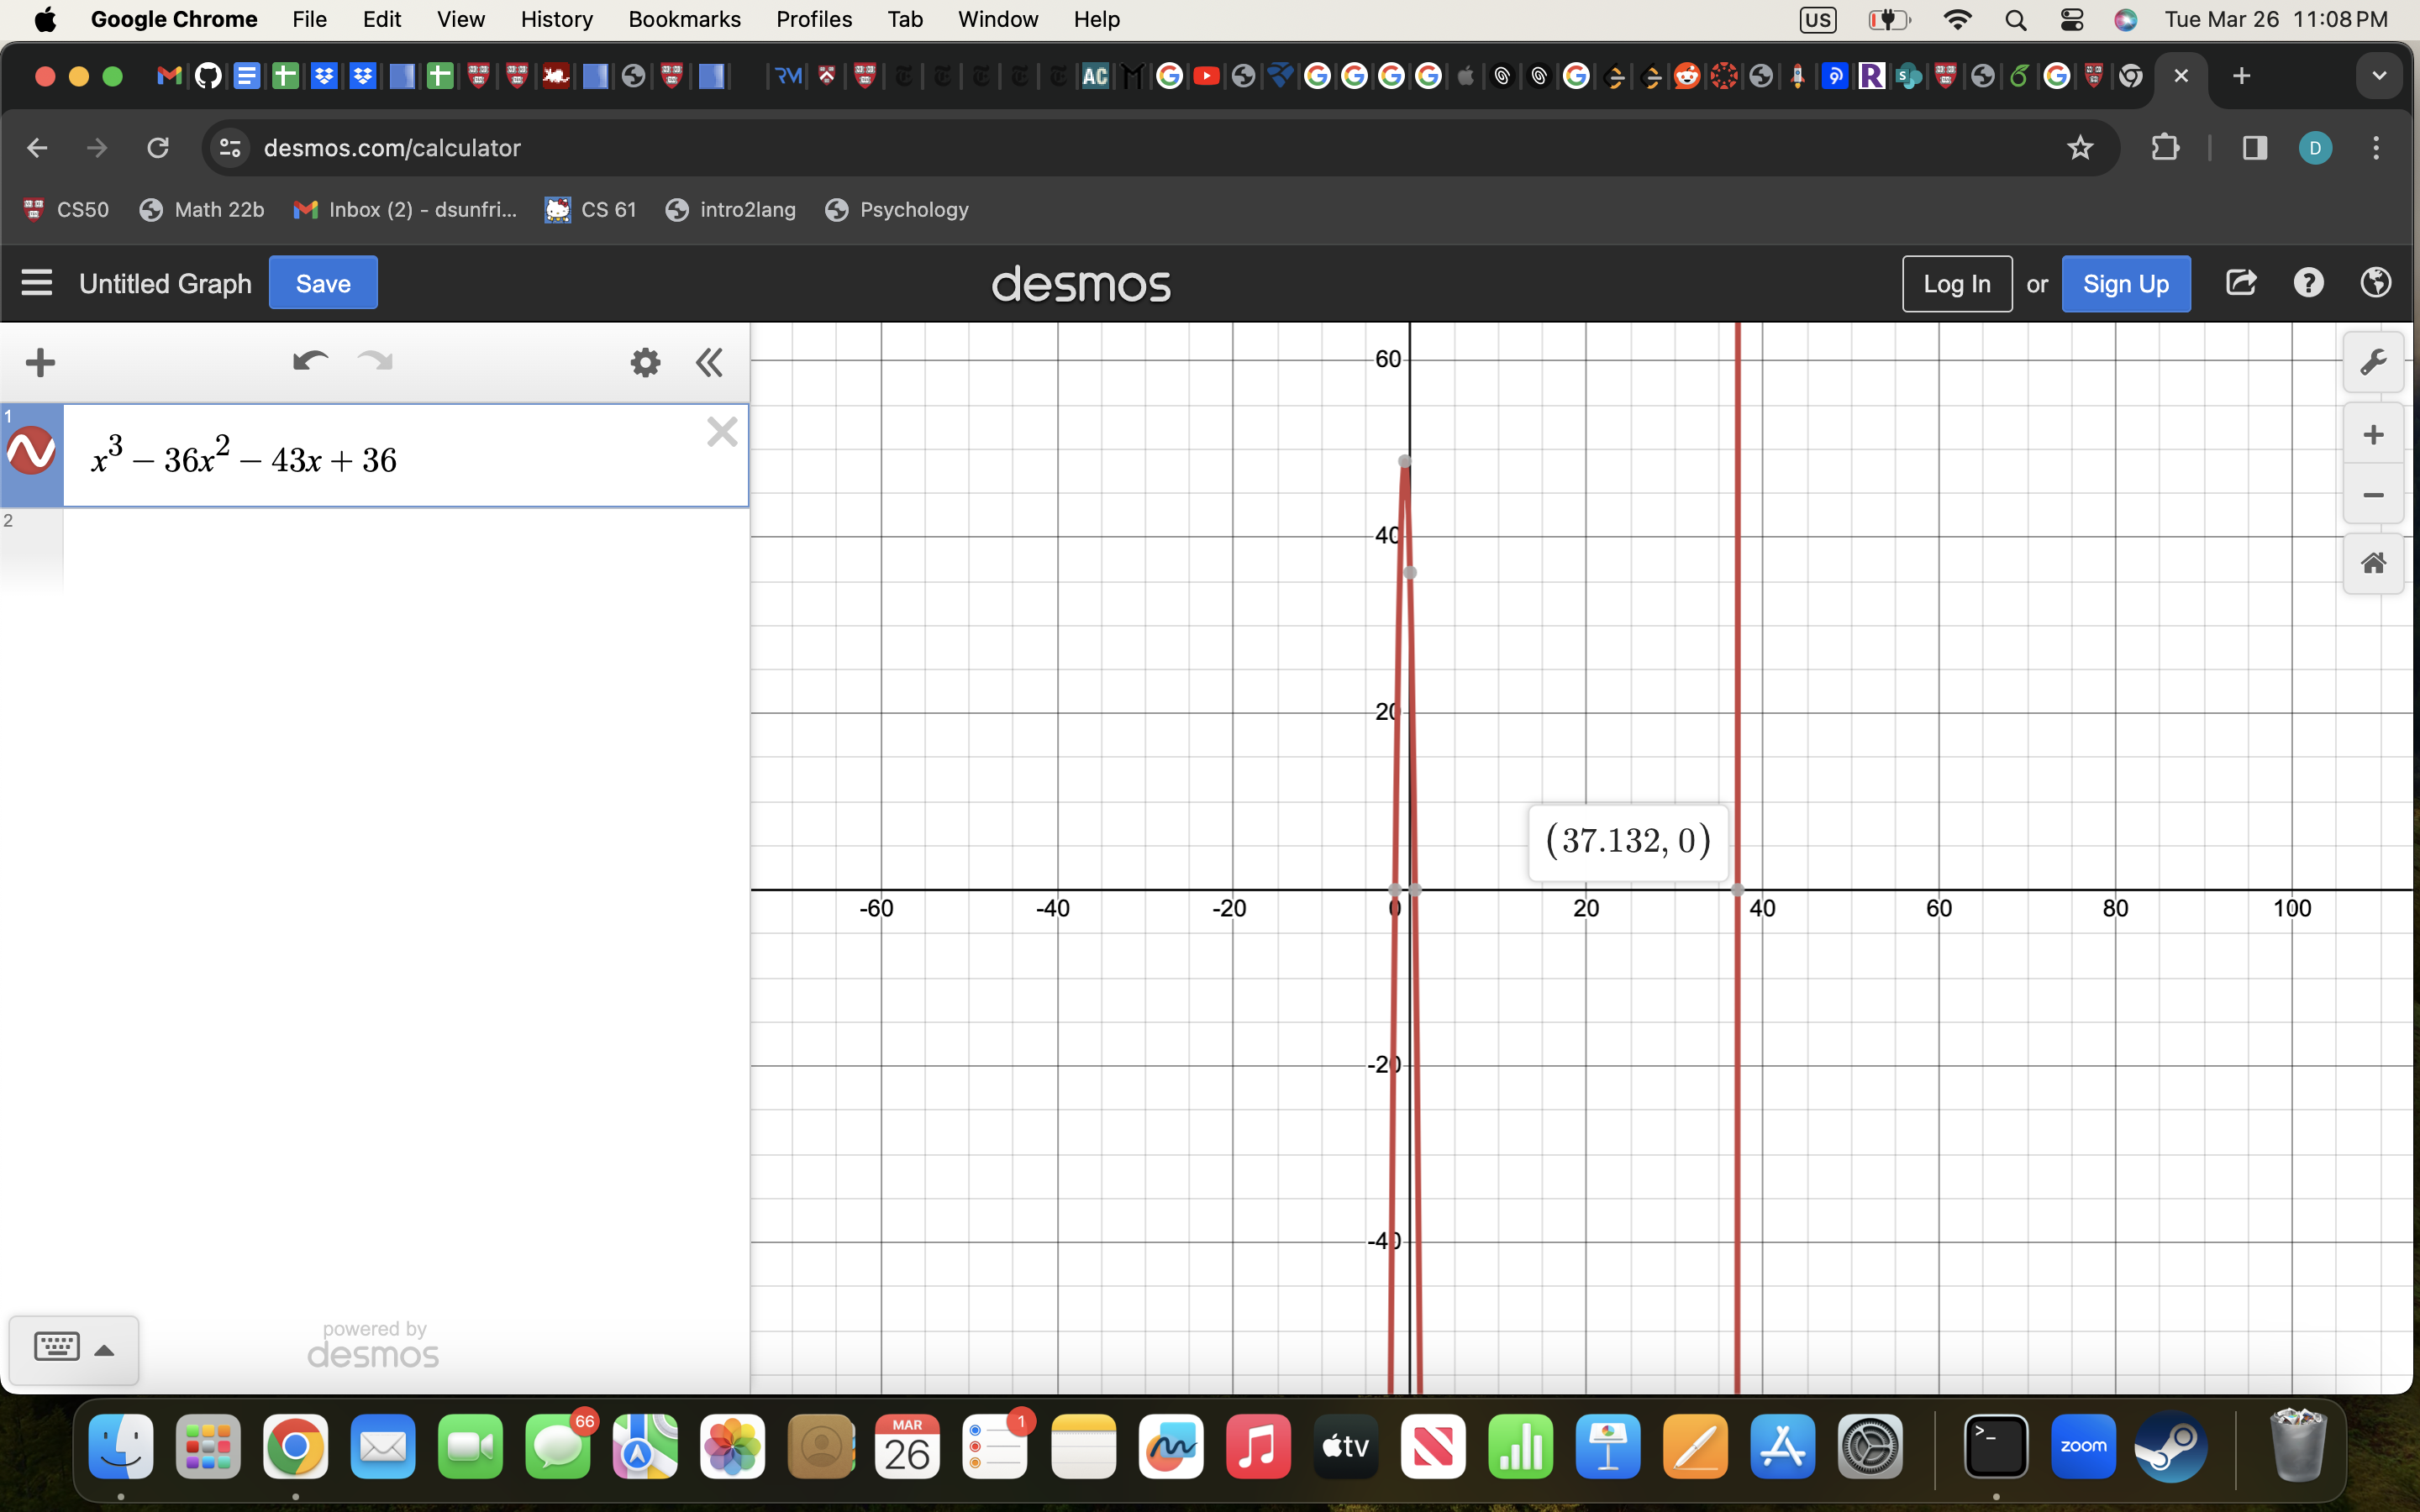
\includegraphics[width=\linewidth]{StrassenPlot.png}

Thus, our final result is that for the even case, the turning point is at $n=15$, and for the odd case, the turning point is at approximately $n=37$.

\section{Section 2: Experimental Analysis}


\section{Section 3: Triangle in Random Graphs}

\end{document}
